% Research Paper for GECCO 2015
% by Nic McPhee, Kirbie Dramdahl, and David Donatucci

\documentclass{sig-alternate}

\usepackage{parskip}
\usepackage{times} %For typeface
\usepackage{graphicx}
\usepackage{algorithm}
\usepackage{algorithm,algorithmic}
\usepackage[justification=centering]{caption}[2007/12/23]
\usepackage{url}
\sloppy

\setlength{\parindent}{0.5cm} 

\newcommand{\citep}[1]{\cite{#1}}

\DeclareGraphicsRule{.tif}{png}{.png}{`convert #1 `dirname #1`/`basename #1 .tif`.png}

\begin{document}

\conferenceinfo{GECCO'15,} {July 11-15, 2015, Madrid, Spain.}
\CopyrightYear{2015}
\crdata{TBA}
\clubpenalty=10000
\widowpenalty = 10000
    
\title{Impact of Crossover Bias in Genetic Programming}

\numberofauthors{1}
\author{
\alignauthor
Nicholas Freitag McPhee, M. Kirbie Dramdahl, David Donatucci\\
	\affaddr{Division of Science and Mathematics}\\
	\affaddr{University of Minnesota, Morris}\\
	\affaddr{Morris, MN USA-56267}\\
	\email{\{mcphee, dramd002, donat056\}@morris.umn.edu}
}

% This is more like how it "should" be done, but I think the previous approach might look nicer. They
% may force us to change it, though, to make it easier to scrape information.

%\numberofauthors{3}
%\author{
%\alignauthor
%Nicholas Freitag McPhee\\
%	\affaddr{Division of Science and Mathematics}\\
%	\affaddr{University of Minnesota, Morris}\\
%	\affaddr{Morris, MN USA-56267}\\
%	\email{mcphee@morris.umn.edu}
%\alignauthor
%M. Kirbie Dramdahl\\
%	\affaddr{Division of Science and Mathematics}\\
%	\affaddr{University of Minnesota, Morris}\\
%	\affaddr{Morris, MN USA-56267}\\
%	\email{dramd002@morris.umn.edu}
%\alignauthor
%David Donatucci\\
%	\affaddr{Division of Science and Mathematics}\\
%	\affaddr{University of Minnesota, Morris}\\
%	\affaddr{Morris, MN USA-56267}\\
%	\email{donat056@morris.umn.edu}
%}

\date{} 
    
\maketitle

\begin{abstract}

\emph{\scriptsize This is probably too long. People often recommend keeping the abstract to somewhere 
between 150 and 250 words, and this is closer to 500. For the initial submission that's OK, but we may want 
to move some of this to the introduction and trim down the abstract somewhat.}

In tree-based genetic programming with sub-tree crossover, the parent contributing the root portion of the tree 
(which 
we refer to as the \emph{root parent}) often contributes more to the semantics of the resulting child than the 
other parent (the 
\emph{non-root parent}). In previous research, we found that when the root parent had greater fitness 
than the 
non-root parent, the fitness of the child tended to be better than if the reverse were true. Here we explore the 
significance of that asymmetry by introducing the notion of \emph{crossover bias}, which allows us to bias the 
system 
in favor of having the more fit parent be the root parent. To better understand the impact of this bias, 
we implemented several levels 
of 
crossover bias, including 0\% bias 
(root individual chosen randomly, as in traditional sub-tree crossover), 
100\% bias (the stronger parent is always chosen to be the root parent), 
50\% bias 
(bias implemented in half 
the cases, and the other half chosen randomly), and reverse bias (the weaker parent is always chosen 
as root parent). 

We applied crossover bias to a variety of problems. In most cases we found that using crossover bias 
either improved performance or had no impact. 
Our results do, however, indicate the possibility that 
crossover bias may increase selection pressure and premature convergence -- undesirable behavior, as it 
encourages a genetic programming run to arrive at a solution too quickly, in the process potentially excluding 
more accurate solutions for a more generalized one.

Our results also demonstrate that the effectiveness of 
crossover bias is somewhat dependent on the problem, and significantly dependent on other parameter 
choices. In 
particular it appears that crossover bias has the largest impact when selection pressure is weaker, and the 
differences 
in the fitness of the parents is thus likely to be larger. We also found that the use of elitism 
reduced the influence of crossover bias. It's possible that crossover bias acts to some degree as an 
``elitism'' operator, making it more likely that the semantics of more fit individuals are copied into the next 
generation; 
thus if traditional elitism is being employed this effect is less visible. Another possible explanation for this is 
that if the most fit individuals are automatically being carried over, there is perhaps less need to produce new, 
fitter individuals via crossover, reducing or even eliminating the usefulness of crossover bias. Other factors 
which we found to have potential impact on the effectiveness of crossover bias were tournament size, 
population size, and possibly the difference in parental fitness.

\end{abstract}

\category{}{}{}
\terms{}
\keywords{genetic programming, crossover bias, root parent}

\section{Introduction} \label{sec:Introduction}

\textbf{Nic should try to capture some nice things Lee Spector said about the importance of asymmetrical 
recombination operators (which are very common in biology, e.g., sex-linked traits) and how we've identified an 
asymmetry in subtree crossover and a way to potentially exploit that.}

\section{Crossover bias} \label{sec:XObias}

\section{Experimental Setup} \label{sec:Experiments}

\textbf{Talk about the fact that we used pairwise Wilcoxon test with Holm corrections for the bulk of our statistical 
tests, along with a reference/citation to R as generated inside R. I'm not sure if we want to mention pairwise test of 
proportions (chi-squared) or not, because I'm not sure how much we'll use it in the paper.}

\section{Results} \label{sec:Results}

\subsection{Structural problems}

\subsubsection{K-Landscapes problems}

We did a full sweep of parameters for the K-Landscapes problem with both $K=2$ and $K=6$.

\begin{itemize}
	\item XO bias of reverse, 0, 0.25, 0.5, 0.75, and 1
	\item Population sizes of 1,024 and 10,240
	\item Elitism of 0\% or 1\%
	\item Tournament sizes of 2, 3, 5, and 7
\end{itemize}

Figure~\ref{fig:KLandscapes6_results} shows the impact of crossover bias on this problem across all the 
combinations of parameter values. Increasing the amount of crossover bias consistently improves the 
fitness of the results. All the differences are statistically significant ($p < 0.012$) except for the difference between
between bias probability 0.75 and 1.0.

%> pairwise.wilcox.test(klandscapes6$Fitness, klandscapes6$Bias.probability)
%
%	Pairwise comparisons using Wilcoxon rank sum test 
%
%data:  klandscapes6$Fitness and klandscapes6$Bias.probability 
%
%     -1      0       0.25    0.5     0.75   
%0    0.99997 -       -       -       -      
%0.25 1.8e-06 1.8e-06 -       -       -      
%0.5  1.7e-12 2.3e-12 0.01136 -       -      
%0.75 < 2e-16 < 2e-16 6.0e-10 0.00032 -      
%1    < 2e-16 < 2e-16 3.7e-15 2.2e-07 0.15773
%
%P value adjustment method: holm 

\begin{figure}
\centering
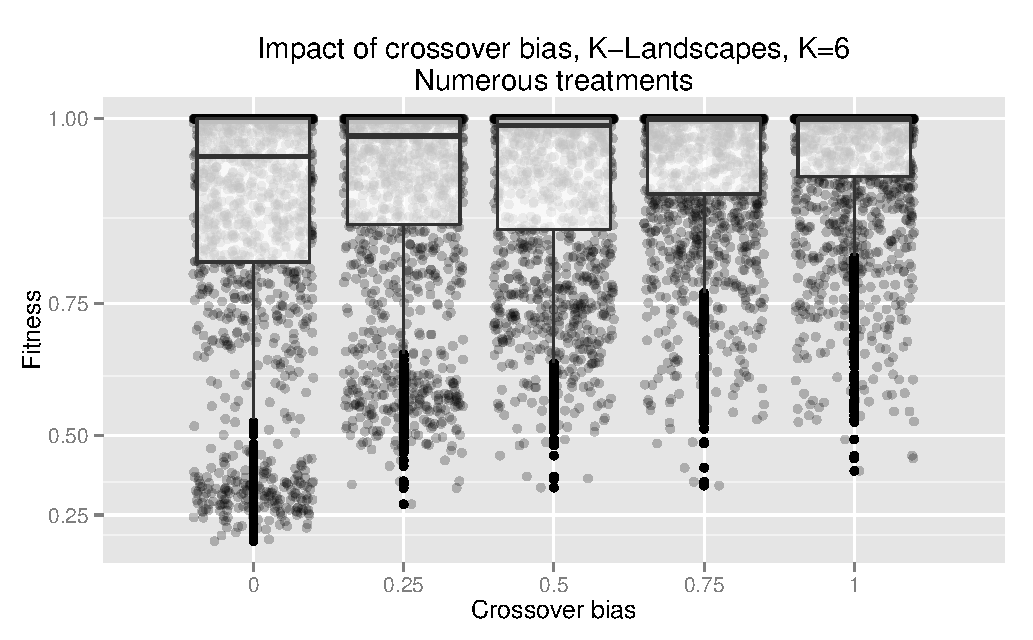
\includegraphics[width=0.45 \textwidth]{Plots/KLandscapes6_XO_bias_impact_transformed_boxplot_alpha075.pdf}
\caption{Impact of crossover bias on fitness for K-Landscapes problem, $K=6$ for a variety of treatments.}
\label{fig:KLandscapes6_results}
\end{figure}

Figure~\ref{fig:KLandscapes6_strong_results} shows the subset set of this information with just binary tournament 
selection, no elitism, and population size of 10,240. It's clear that the impact of crossover bias is much stronger in this 
case than in the more general case shown in Figure~\ref{fig:KLandscapes6_results}. Here all the differences are strongly 
statistically significant ($p < 10^{-11}$) except for the difference between reverse bias (-1) and no bias (0). Increasing 
the crossover bias increases the number of ``perfect'' solutions discovered as well as just increasing the fitness. 15 
solutions were discovered in the 100 runs with crossover bias at 1.0, where only 1 or 2 solutions were discovered for 
each of the other crossover bias probabilities; this difference is statistically significant with $p \leq 0.03$ using a 
pairwise test of proportions.

\begin{figure}
\centering
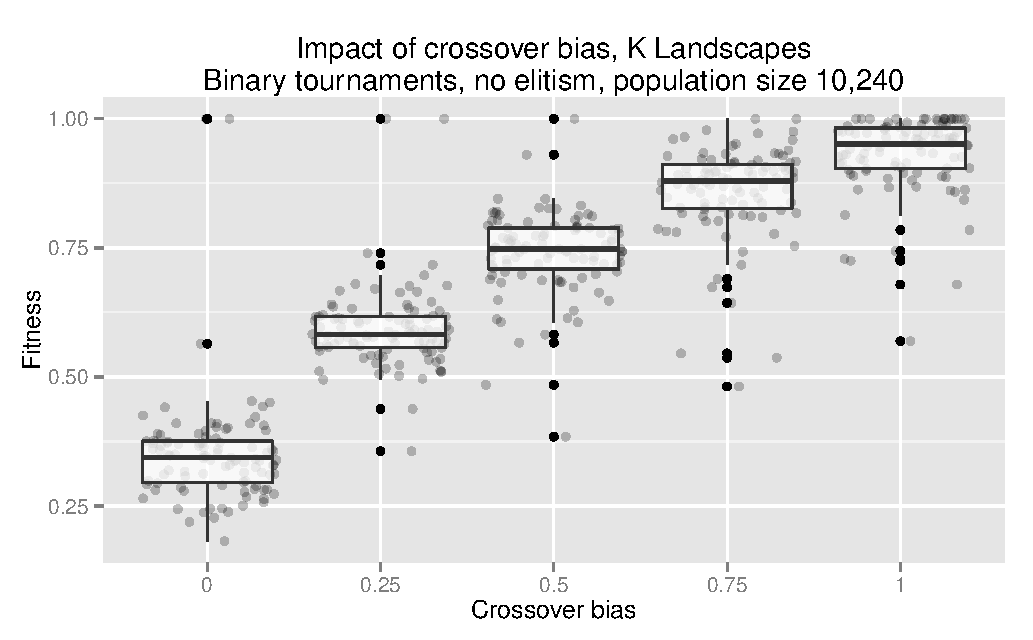
\includegraphics[width=0.45 \textwidth]{Plots/KLandscapes6_XO_bias_strong_impact_alpha_075.pdf}
\caption{Impact of crossover bias on fitness for K-Landscapes problem, $K=6$, restricted to binary tournament 
selection, no elitism, and population size 10,240.}
\label{fig:KLandscapes6_strong_results}
\end{figure}

%> pairwise.wilcox.test(strong$Fitness, strong$Bias.probability)
%
%	Pairwise comparisons using Wilcoxon rank sum test 
%
%data:  strong$Fitness and strong$Bias.probability 
%
%     -1      0       0.25    0.5     0.75   
%0    0.18    -       -       -       -      
%0.25 < 2e-16 < 2e-16 -       -       -      
%0.5  < 2e-16 < 2e-16 < 2e-16 -       -      
%0.75 < 2e-16 < 2e-16 < 2e-16 < 2e-16 -      
%1    < 2e-16 < 2e-16 < 2e-16 < 2e-16 2.3e-12
%
%P value adjustment method: holm 

%> countSuccesses(strong)
%[1]  1  2  2  1  2 15
%> pairwise.prop.test(countSuccesses(strong), rep(100, 6))
%
%	Pairwise comparisons using Pairwise comparison of proportions 
%
%data:  countSuccesses(strong) out of rep(100, 6) 
%
%  1     2     3     4     5    
%2 1.000 -     -     -     -    
%3 1.000 1.000 -     -     -    
%4 1.000 1.000 1.000 -     -    
%5 1.000 1.000 1.000 1.000 -    
%6 0.011 0.030 0.030 0.011 0.030
%
%P value adjustment method: holm 

\subsubsection{Ordertree problem}

\textbf{Everything in this section at the moment is really just Nic chatting about the results that we have, hoping for 
some ideas/feedback from Kirbie and David. Thoughts, suggestions, questions, changes, actual usable text, etc., all 
greatly appreciated.}

We have two groups of Ordertree results, the first from November 2014, and the second from January 20145. The 
earlier results just varied the tournament size and the bias probability, leaving the population size at 500 (the default in 
ECJ for that problem) and no elitism (also the default). Those results are where Figures~\ref{fig:Ordertree_results} 
and~\ref{fig:Ordertree_results_binary_tournaments} come from. These plots are nice and ``clean'' and say what we 
want to say without complicating things.

\begin{figure}
\centering
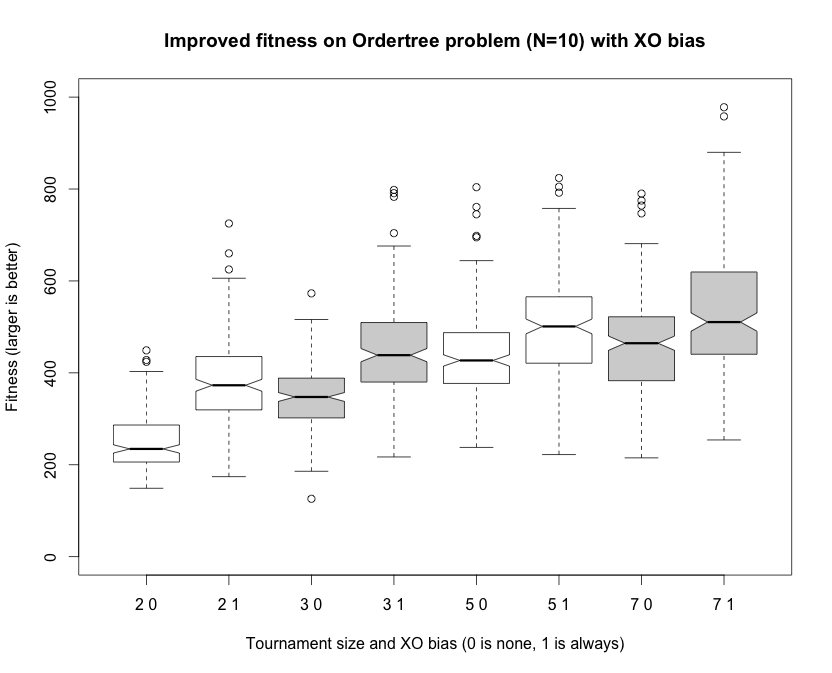
\includegraphics[width=0.45 \textwidth]{Plots/Ordertree_results.png}
\caption{Impact of crossover bias on fitness for Ordertree problem for various tournament sizes. \textbf{Redraw this 
as PDF and mention how improvement drops as tournament sizes grow.}}
\label{fig:Ordertree_results}
\end{figure}

\begin{figure}
\centering
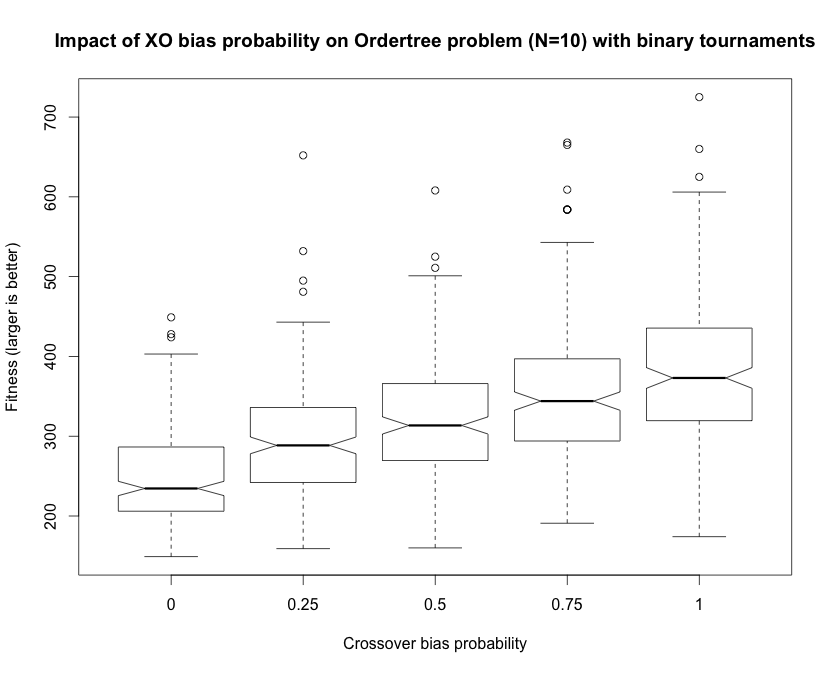
\includegraphics[width=0.45 \textwidth]{Plots/Ordertree_XO_bias_prob_binary_tournaments.png}
\caption{Impact of crossover bias on fitness for Ordertree problem for binary tournaments.}
\label{fig:Ordertree_results_binary_tournaments}
\end{figure}

The later runs are more in keeping with what we'd been doing on other problems. They do a full sweep of bias 
probabilities, all four tournament sizes (2, 3, 5, and 7), and with and without elitism (1\% when used). The population 
size was only 1,024 because the trees get really big for this problem and we'd run out of memory if we used 10K 
pops.

The rub is that the results are different with the larger populations, and it's not clear how we want to handle this in the 
paper. In particular, the fitnesses are actually a little \emph{worse} for bias 1.0 than for bias 0.75, i.e., the performance 
``curve'' goes up and then begins to dip down.

Figure~\ref{fig:Ordertree_results_Jan15_facets} shows the results of runs both with and without crossover bias (i.e,. 
crossover bias probability either 1 or 0) for all four tournament sizes, and in each case adding crossover bias 
improves fitness. All these differences are statistically significant ($p < 0.002$ for each pairing using a pairwise 
Wilcoxon with Holm correction).

\begin{figure}
\centering
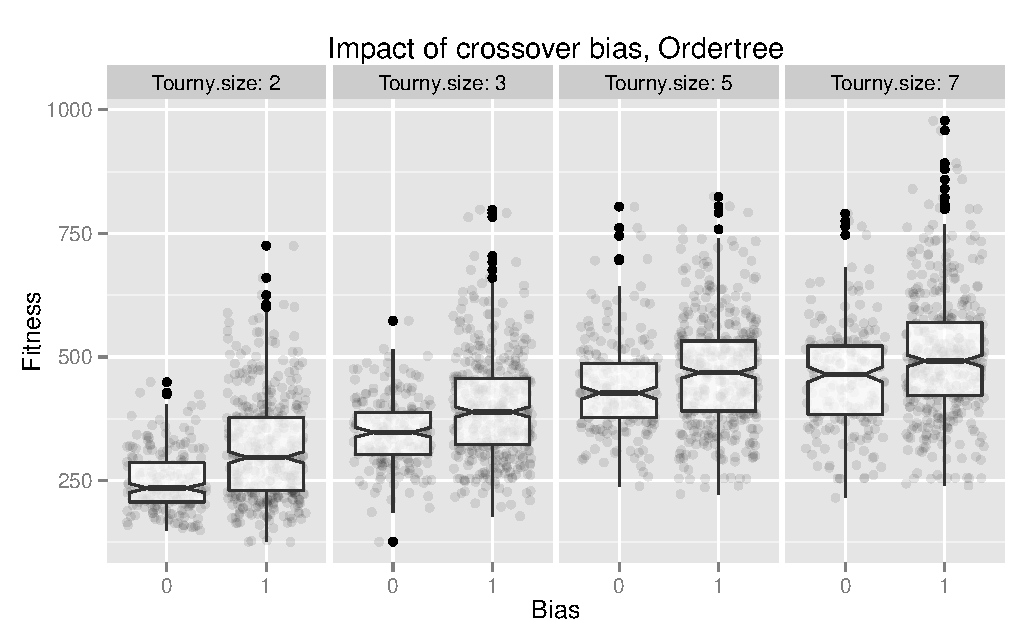
\includegraphics[width=0.45 \textwidth]{Plots/Ordertree_results_Jan15_facets.pdf}
\caption{Impact of crossover bias on fitness for Ordertree problem for various tournament sizes.}
\label{fig:Ordertree_results_Jan15_facets}
\end{figure}

Figure~\ref{fig:Ordertree_results_binary_tournaments_Jan15} shows the impact of a range of crossover bias values 
limited to binary tournaments. Here we see the drop in fitness for bias 1.0, actually dropping slightly below that for 0.5 
as well as 0.75. All these differences are statistically significant ($p < 0.03$) except for the difference between bias 
0.25 and bias 1.0, so bias of 0.75 is the clear winner here. \textbf{I (Nic) suspect this is actually quite interesting and 
might open interesting doors to things like premature convergence and need for being able to have a least a little 
variation in the system for a problem like this. Maybe we should talk about that in the "Future work" section?} Figure~
\ref{fig:Ordertree_results_all_tournaments_Jan15} generalizes this to cover all four tournament sizes (so the leftmost 
panel of this figure is essentially the preceding figure). Here we see that the fitness drops for bias 1.0 for all four 
tournament sizes. In general the impact of crossover bias lessens with the larger tournament sizes, both in the 
increase in fitness up to bias 0.75, and the drop from there to bias 1.0.

\begin{figure}
\centering
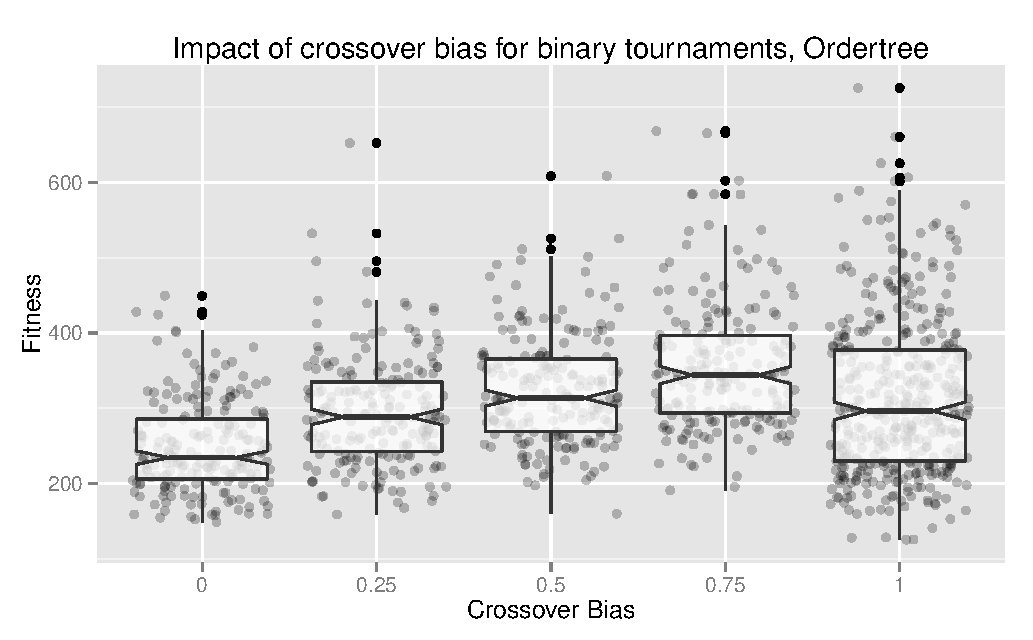
\includegraphics[width=0.45 \textwidth]{Plots/Ordertree_results_binary_tournaments_Jan15.pdf}
\caption{Impact of crossover bias on fitness for Ordertree problem for binary tournaments.}
\label{fig:Ordertree_results_binary_tournaments_Jan15}
\end{figure}

\begin{figure}
\centering
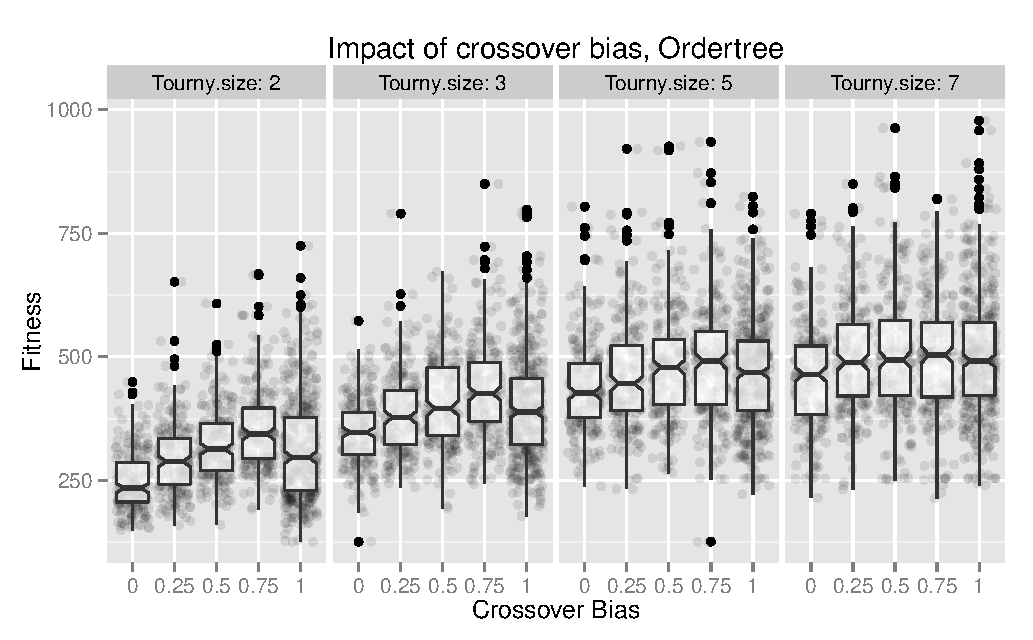
\includegraphics[width=0.45 \textwidth]{Plots/Ordertree_results_all_tournaments_Jan15.pdf}
\caption{Impact of crossover bias on fitness for Ordertree problem for multiple tournament sizes.}
\label{fig:Ordertree_results_all_tournaments_Jan15}
\end{figure}

Just to check that this wasn't happening everywhere, Figure~\ref{fig:KLandscapes6_XO_bias_impact_facets} plots 
the corresponding data from the K-Landscapes runs. It's clear that for binary tournaments, increasing the crossover 
bias probability continues to improve the fitness. This continues to be true for tournament size 3. For tournament 7, 
however, it does look like the reverse is true, where increasing crossover actually hurts fitness. Almost none of the 
differences for tournament size 7 are statistically significant, however, with the only exception being the difference 
between 0.25 and 1.0 ($p=0.21$ using a pairwise Wilcoxon test with Holm correction). \textbf{This paragraph might 
move to the Discussion or Conclusions section if we keep it, or something like it.}

% None of the differences are significant for tourney size 5. All the differences are significant for TS=3 except for bias 
0.5 and 0.75 and that was very close ($p=0.05620$). All the differences for binary are \emph{strongly} significant 
($p<6e-08$).

\begin{figure}
\centering
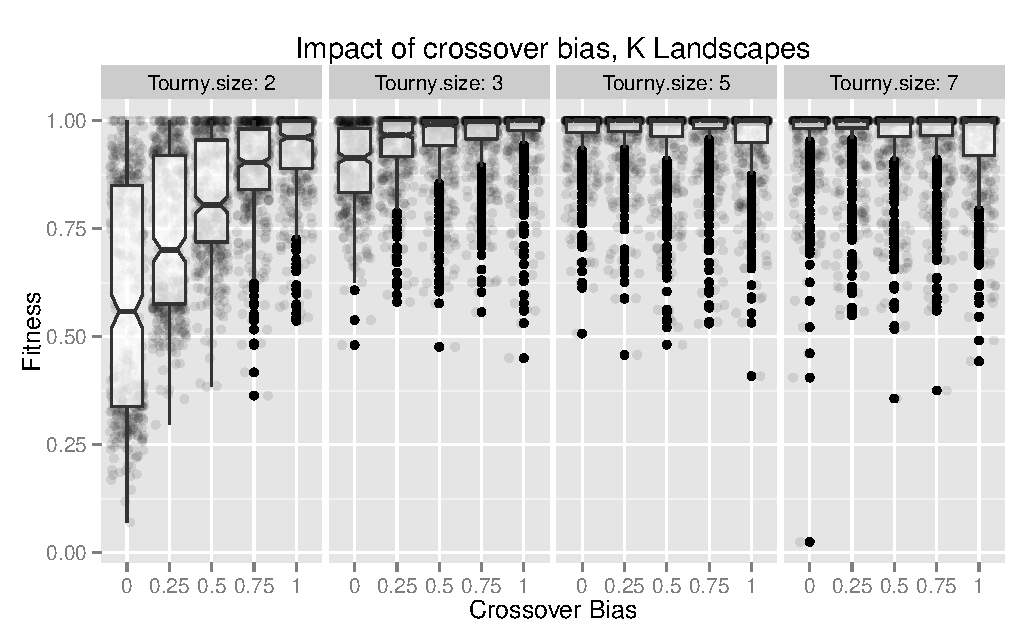
\includegraphics[width=0.45 \textwidth]{Plots/KLandscapes6_XO_bias_impact_facets.pdf}
\caption{Impact of crossover bias on fitness for K-Landcapes problem, K=6, for various tournament sizes.}
\label{fig:KLandscapes6_XO_bias_impact_facets}
\end{figure}

%> pairwise.wilcox.test(subset(klandscapes6, Tourny.size==7)$Fitness, subset(klandscapes6, Tourny.size==7)$Bias.probability)
%
%	Pairwise comparisons using Wilcoxon rank sum test 
%
%data:  subset(klandscapes6, Tourny.size == 7)$Fitness and subset(klandscapes6, Tourny.size == 7)$Bias.probability 
%
%     0     0.25  0.5   0.75 
%0.25 1.000 -     -     -    
%0.5  1.000 1.000 -     -    
%0.75 1.000 0.556 1.000 -    
%1    0.075 0.021 0.556 1.000
%
%P value adjustment method: holm 

\subsection{U.S. Change problem}

For the U.S. Change problem, we'll use ``Hits'' (the number of test cases that are correctly solved) as the measure of 
the success of a run. There are 150 test cases in our implementation, so an optimal program will have a ``Hits'' score 
of 150.

Figure~\ref{fig:USChange_Hits} shows the impact of crossover bias on the number of hits for the U.S. Change 
problem across the full collection of parameter settings. This suggests that in in general there is little consistent 
impact of crossover bias, but a pairwise Wilcoxon test with Holm correction indicates that while most of the 
differences in this plot aren't statistically significant, two are: The differences between crossover bias 0 and crossover 
bias 0.5 and 0.75 are both statistically significant ($p \leq 0.015$), even if numerically small.

\begin{figure}
\centering
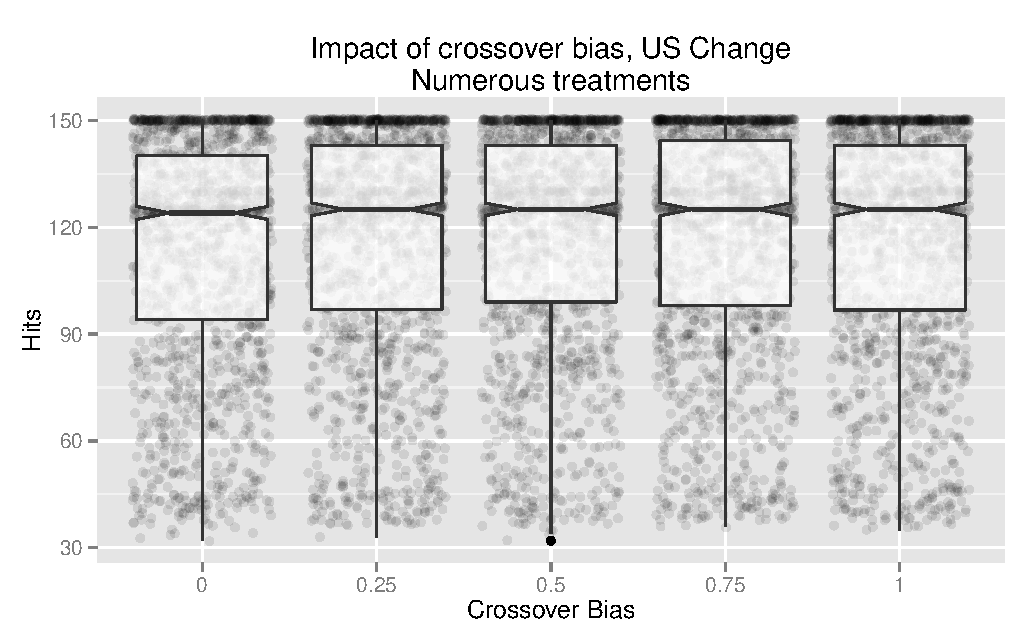
\includegraphics[width=0.45 \textwidth]{Plots/US_change_hits.pdf}
\caption{Impact of crossover bias on the number of hits for the US Change problem.}
\label{fig:USChange_Hits}
\end{figure}

%> pairwise.wilcox.test(us_change$Hits, us_change$Bias, conf.int=TRUE)
%
%	Pairwise comparisons using Wilcoxon rank sum test 
%
%data:  us_change$Hits and us_change$Bias 
%
%     0     0.25  0.5   0.75 
%0.25 0.117 -     -     -    
%0.5  0.011 1.000 -     -    
%0.75 0.015 1.000 1.000 -    
%1    0.083 1.000 1.000 1.000
%
%P value adjustment method: holm 

If we limit our attention to binary tournaments, no elitism, and the larger population size (10,240), then we find that 
crossover bias has a substantial and statistically significant impact, as is seen in Figure~
\ref{fig:USChange_Hits_strong}. Here the bulk of these pairwise differences are statistically significant ($p<0.0002$ 
using a pairwise Wilcoxon test with Holm correction). The major exception is the difference between crossover bias 
0.75 and 1.0 ($p=0.43078$). Two other adjacent pairs have $p$-values slightly above 0.05: Crossover bias 0.25 
\emph{vs.} 0.5 ($p=0.05036$), and 0.5 \emph{vs.} 0.75 ($p=0.08019$). \textbf{We could put all the $p$ values in a 
table, bolding the ones that are significant. This is somewhat common in the literature, but would use quite a bit more 
space, especially since half the table would be empty. Thoughts?}

\begin{figure}
\centering
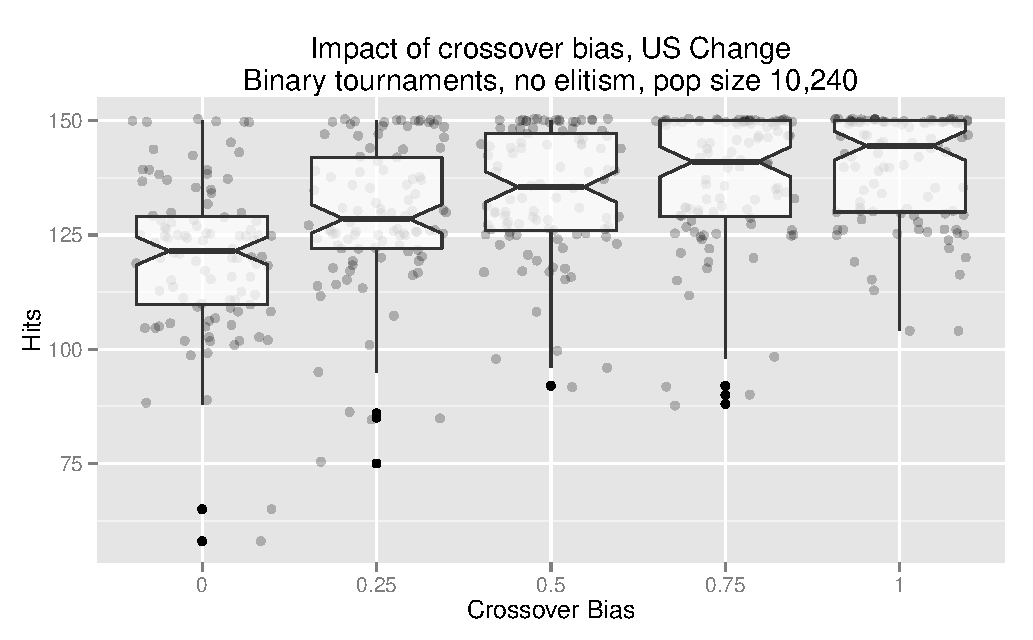
\includegraphics[width=0.45 \textwidth]{Plots/US_change_hits_strong.pdf}
\caption{Impact of crossover bias on the number of hits for the US Change problem, limited to binary 
tournaments, no elitism, and population size 10,240.}
\label{fig:USChange_Hits_strong}
\end{figure}

%> pairwise.wilcox.test(us_change_strong$Hits, us_change_strong$Bias)
%
%	Pairwise comparisons using Wilcoxon rank sum test 
%
%data:  us_change_strong$Hits and us_change_strong$Bias 
%
%     0       0.25    0.5     0.75   
%0.25 0.00013 -       -       -      
%0.5  3.4e-09 0.05036 -       -      
%0.75 1.1e-12 0.00016 0.08019 -      
%1    3.2e-15 5.1e-06 0.01652 0.43078
%
%P value adjustment method: holm 

If complete success was considered vital (which might be the case if we were evolving software for use in a 
production system), then it would make sense to see if crossover bias has a significant impact on the success rate. 
Figure~\ref{fig:USChange_Successes_strong} shows the number of successes for the various crossover bias values 
when using binary tournaments, no elitism, and population size 10.240. A pairwise test of proportions (chi-squared) 
with Holm correction indicates that while non of the adjacent differences (e.g., crossover bias 0.5 \emph{vs.} 0.75) are 
statistically significant, most of the non-adjacent differences (e.g., crossover bias 0.25 \emph{vs.} 0.75) are 
statistically significant, with the exceptions being crossover bias 0 \emph{vs.} 0.5, and bias 0.5 and 1.0 ($p=0.09361$ 
in both cases). 

\begin{figure}
\centering
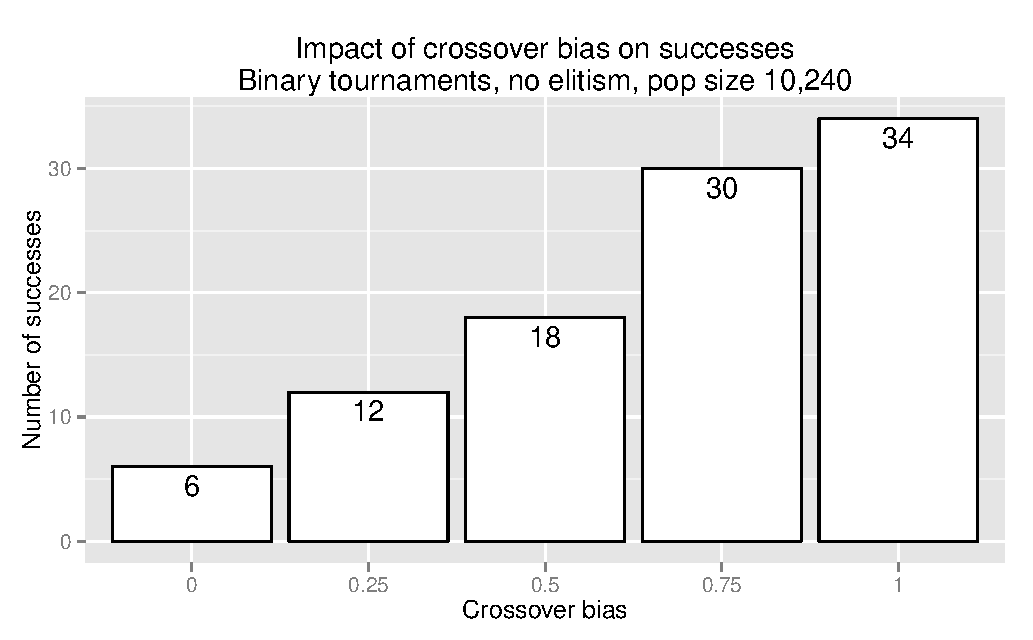
\includegraphics[width=0.45 \textwidth]{Plots/US_change_successes_strong.pdf}
\caption{Impact of crossover bias on the number of successes runs for the US Change problem when using 
binary tournaments, no elitism, and population size 10,240.}
\label{fig:USChange_Successes_strong}
\end{figure}

%> pairwise.prop.test(c(6, 12, 18, 30, 34), rep(100, 5))
%
%	Pairwise comparisons using Pairwise comparison of proportions 
%
%data:  c(6, 12, 18, 30, 34) out of rep(100, 5) 
%
%  1       2       3       4      
%2 0.65003 -       -       -      
%3 0.09361 0.65003 -       -      
%4 0.00021 0.02215 0.27429 -      
%5 1.8e-05 0.00334 0.09361 0.65003
%
%P value adjustment method: holm 

%\begin{figure}
%\centering
%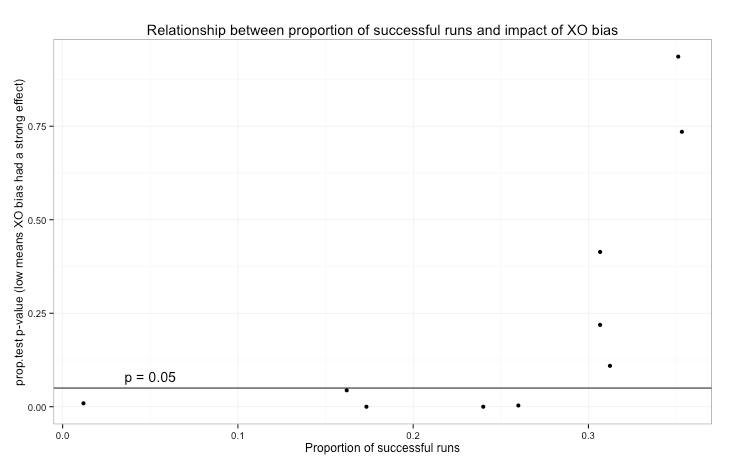
\includegraphics[width=0.45 \textwidth]{Plots/US_change_Bias_impact_vs_success.png}
%\caption{Relationship between proportion of successful runs and the impact of crossover bias.}
%\label{fig:USChangeBiasImpactVsSuccess}
%\end{figure}

\subsection{Symbolic regression problems}

\subsubsection{Pagie-1 problem}

\begin{figure}
\centering
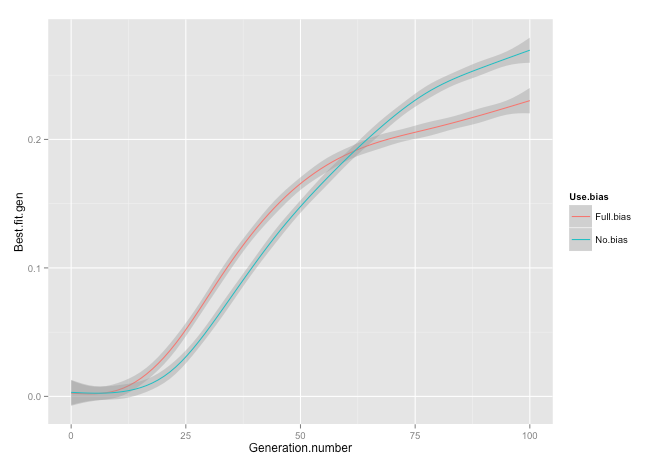
\includegraphics[width=0.45 \textwidth]{Plots/Pagie-1_fitness_vs_time.png}
\caption{Impact of crossover bias on the fitness over time for the Pagie-1 symbolic regression problem}
\label{fig:Pagie1FitnessOverTime}
\end{figure}

\begin{figure}
\centering
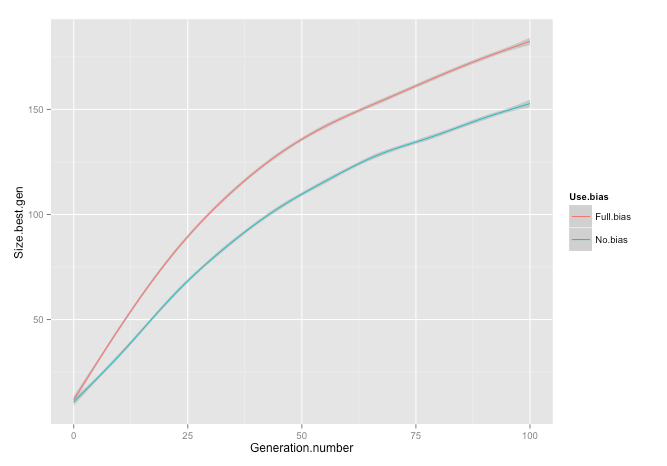
\includegraphics[width=0.45 \textwidth]{Plots/Pagie-1_size_vs_time.png}
\caption{Impact of crossover bias on the tree size over time for the Pagie-1 symbolic regression problem}
\label{fig:Pagie1SizeOverTime}
\end{figure}

\begin{figure}
\centering
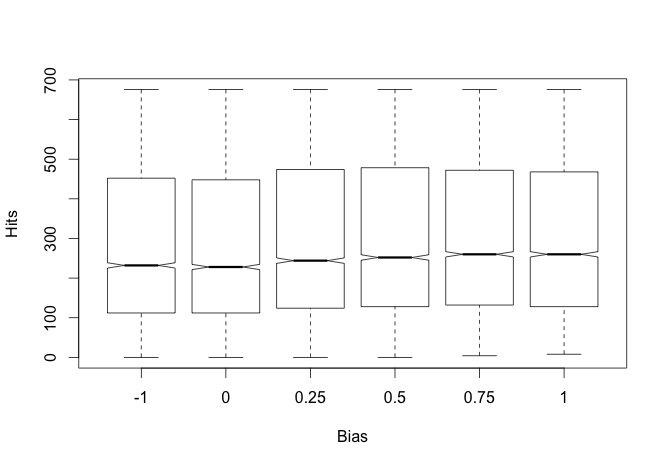
\includegraphics[width=0.45 \textwidth]{Plots/Pagie-1_Hits_vs_Bias.png}
\caption{Impact of crossover bias on the number of hits for the Pagie-1 symbolic regression problem. 
Unfortunately I'm not immediately sure what (sub)set of data this includes.}
\label{fig:Pagie1Hits}
\end{figure}

\begin{figure}
\centering
\includegraphics[width=0.45 \textwidth]{Plots/Pagie-1_Successes_vs_Bias.png}
\caption{Impact of crossover bias on the number of successes (runs that exactly solve the problem) for the 
Pagie-1 symbolic regression problem. Unfortunately I'm not immediately sure what (sub)set of data this 
includes.}
\label{fig:Pagie1Successes}
\end{figure}

\begin{figure}
\centering
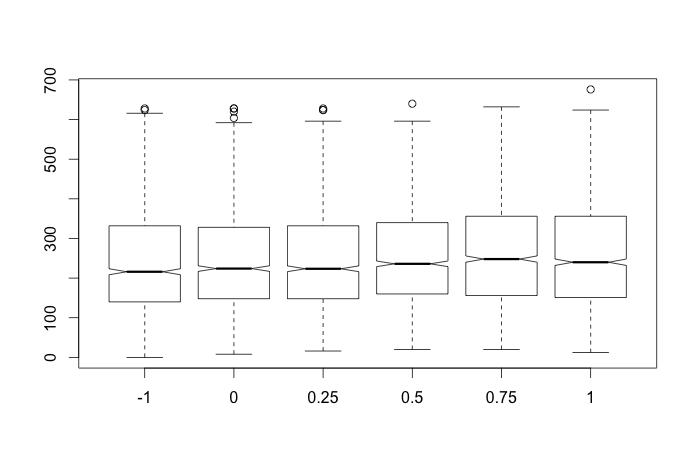
\includegraphics[width=0.45 \textwidth]{Plots/Pagie-1-koza2_no_Tarpeian.png}
\caption{Impact of crossover bias on the number of hits when using the koza2 function set for the Pagie-1 
symbolic regression problem.}
\label{fig:Pagie1Koza2}
\end{figure}

\begin{figure}
\centering
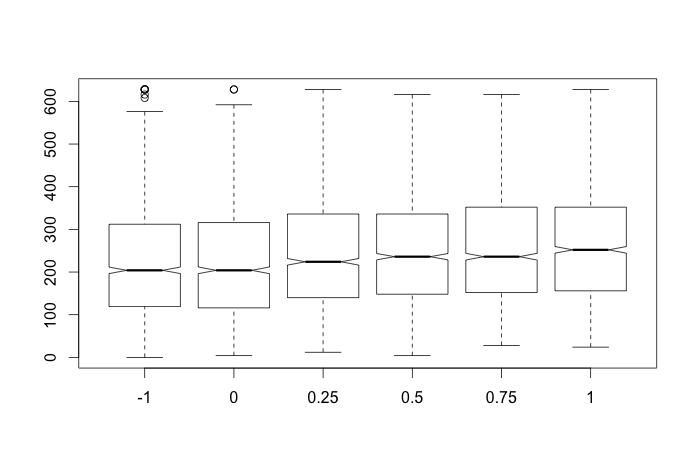
\includegraphics[width=0.45 \textwidth]{Plots/Pagie-1-tarp.png}
\caption{Impact of crossover bias on the number of hits when using the koza2 function set and Tarpeian bloat 
control for the Pagie-1 symbolic regression problem.}
\label{fig:Pagie1Koza2Tarpeian}
\end{figure}

\subsubsection{Sine problem}

Figure~\ref{fig:sineBiasResultsStrong} shows the hits results for the sine regression problem using binary tournaments, no 
elitism, and population size 10,240. All these differences are statistically significant ($p < 10^{-5}$ using a 
pairwise Wilcoxon rank sum test) except for the difference between the bias of 0.75 and 1.0.

\begin{figure}
\centering
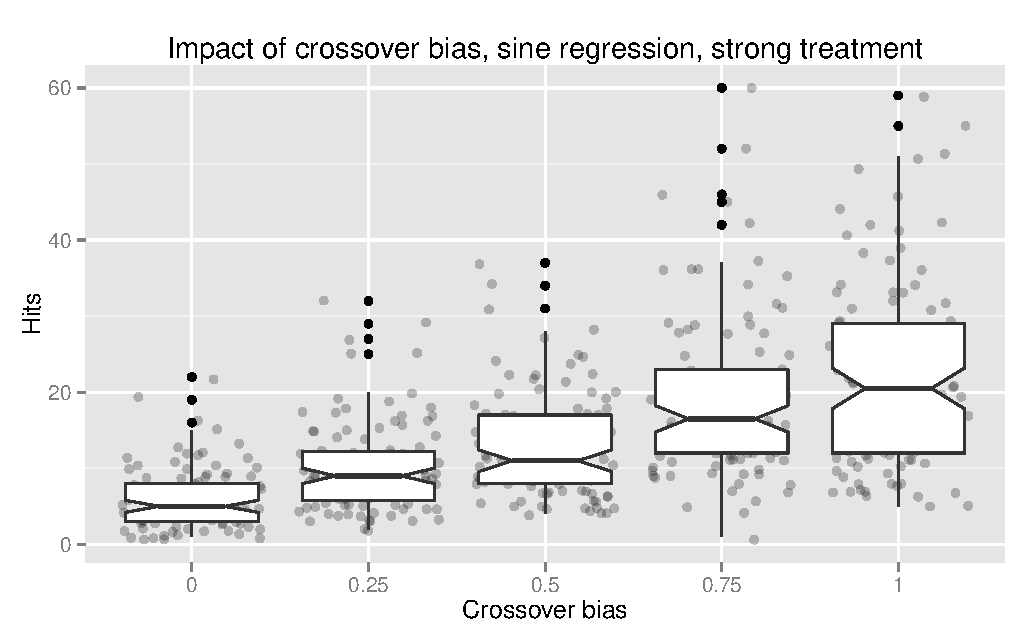
\includegraphics[width=0.45 \textwidth]{Plots/Sine_XO_impact_strong_boxplot.pdf}
\caption{Impact of crossover bias on the sine symbolic regression problem with binary tournaments, no elitism, and 
population size 10,240}
\label{fig:sineBiasResultsStrong}
\end{figure}

%> pairwise.wilcox.test(sine_strong_final$Hits, sine_strong_final$Bias)
%
%	Pairwise comparisons using Wilcoxon rank sum test 
%
%data:  sine_strong_final$Hits and sine_strong_final$Bias 
%
%     0       0.25    0.5     0.75  
%0.25 1.9e-07 -       -       -     
%0.5  4.0e-15 0.0017  -       -     
%0.75 < 2e-16 1.2e-12 8.9e-06 -     
%1    < 2e-16 1.3e-13 2.9e-07 0.1938
%
%P value adjustment method: holm 

%> pairwise.wilcox.test(sine_strong_final$Standardized.fitness, sine_strong_final$Bias)
%
%	Pairwise comparisons using Wilcoxon rank sum test 
%
%data:  sine_strong_final$Standardized.fitness and sine_strong_final$Bias 
%
%     0       0.25    0.5     0.75 
%0.25 3.6e-10 -       -       -    
%0.5  < 2e-16 2.7e-05 -       -    
%0.75 < 2e-16 5.0e-14 1.1e-05 -    
%1    < 2e-16 < 2e-16 2.9e-09 0.072
%
%P value adjustment method: holm 

Figure~\ref{fig:sineBiasResultsWeak} shows the results for the sine regression problem using tournament size 7, 0.1\% 
elitism, and smaller populations  of size 1,024. None of these differences are statistically significant using a 
pairwise Wilcoxon rank sum test.

\begin{figure}
\centering
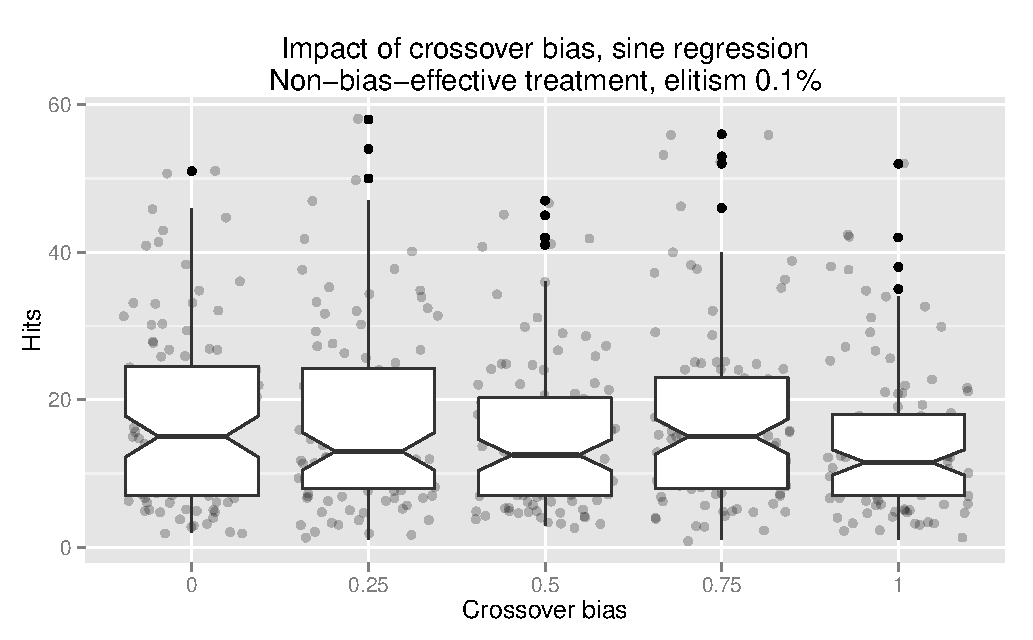
\includegraphics[width=0.45 \textwidth]{Plots/Sine_XO_impact_weak_boxplot.pdf}
\caption{Impact of crossover bias on the sine symbolic regression problem with tournament size 7, 0.1\% elitism, and 
population size 1,024.}
\label{fig:sineBiasResultsWeak}
\end{figure}

Figures~\ref{fig:sineBiasFitnessVsGenStrong} and~\ref{fig:sineBiasFitnessVsGenWeak} show the change in fitness 
over time for the strong and weak configurations. In the strong configuration we get a really clean ``adding bias is 
good'' demonstration. In the weak configuration, the impact of crossover bias is quite minimal; \textbf{oddly, though, it 
does look like a crossover bias of 1.0 is worse by a little bit than everything else at the end, which is weird}. Figure~
\ref{fig:sineBiasFitnessVsGenT2E01P10K} shows fitness over time for the ``weak'' configuration with population size 
10,240 (instead of 1,024 for the ``normal'' weak configuration). Increasing the pop size definitely improves the 
performance by quite a lot (no surprise). The different bias levels are all essentially the same at the end of the 100 
generations, but there is definitely a spread around 15-20 generations that is a really clean ``more bias is better'' 
demonstration (\textbf{Do we care?}) except for the fact that 0.75 and 1.0 are essentially the same. \textbf{Do we 
want to include both Figures~\ref{fig:sineBiasFitnessVsGenWeak} and~\ref{fig:sineBiasFitnessVsGenT2E01P10K}? 
Do we want to combine them into a single graph (either just one graph, or as two ``panels'' like, e.g., in Figure~
\ref{fig:parentErrorsSine}?}

\begin{figure}
\centering
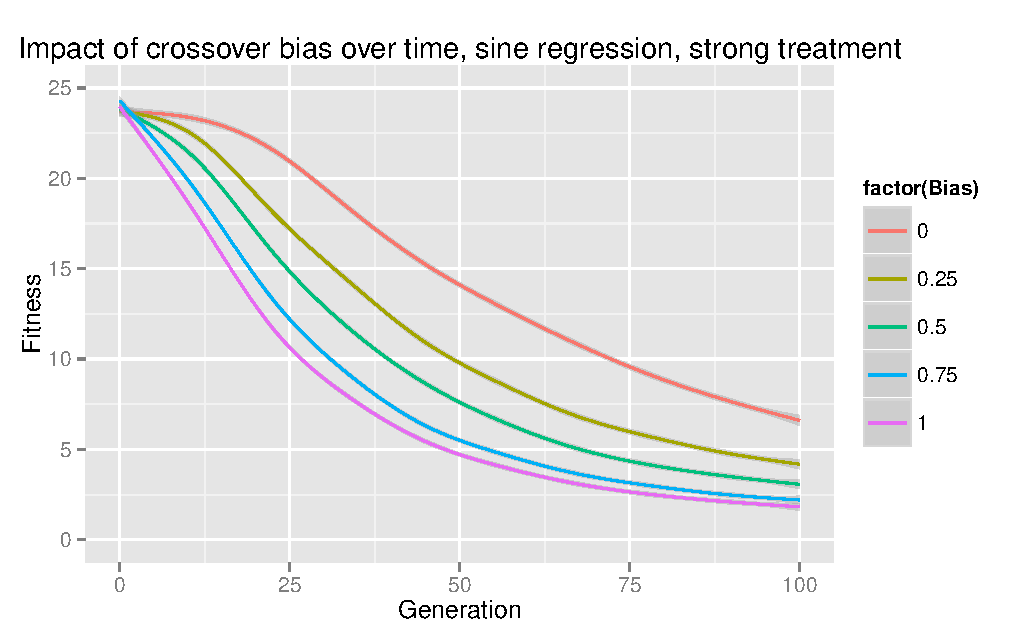
\includegraphics[width=0.45 \textwidth]{Plots/Sine_XO_fitness_vs_gen_strong.pdf}
\caption{Impact of crossover bias on the sine symbolic regression problem with binary tournaments, no elitism, and 
population size 10,240.}
\label{fig:sineBiasFitnessVsGenStrong}
\end{figure}

\begin{figure}
\centering
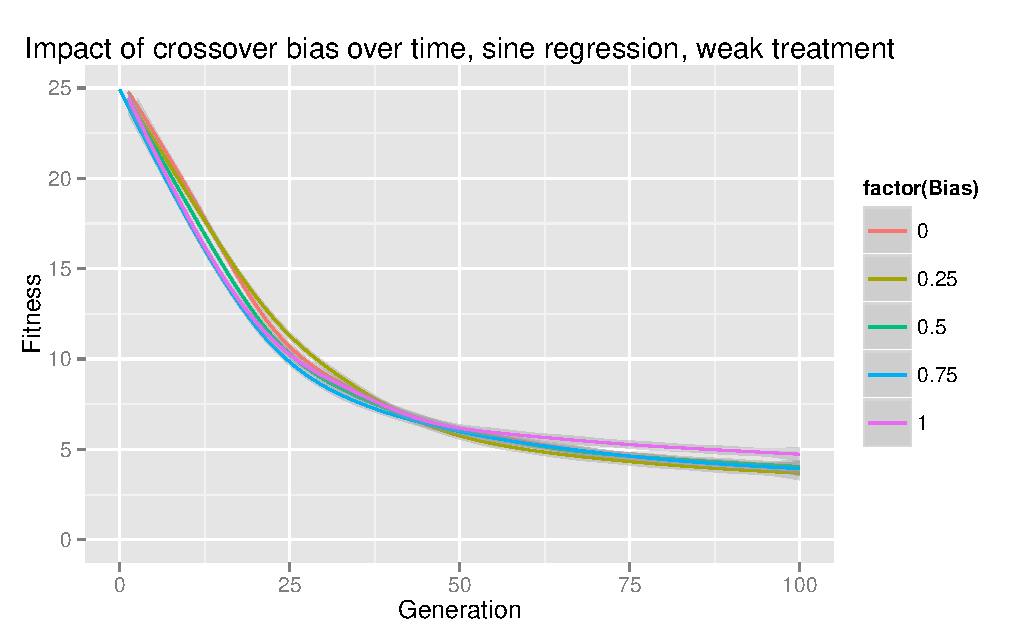
\includegraphics[width=0.45 \textwidth]{Plots/Sine_XO_fitness_vs_gen_weak.pdf}
\caption{Impact of crossover bias on the sine symbolic regression problem with tournament size 7, 0.1\% elitism, and 
population size 1,024.}
\label{fig:sineBiasFitnessVsGenWeak}
\end{figure}

\begin{figure}
\centering
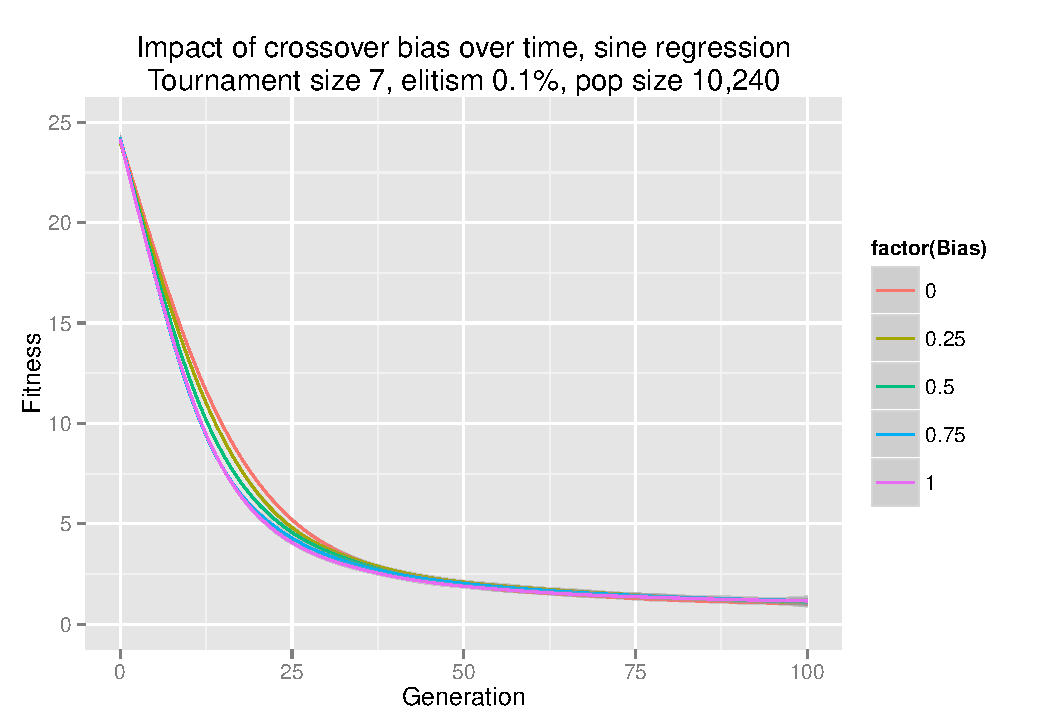
\includegraphics[width=0.45 \textwidth]{Plots/Sine_XO_fitness_vs_gen_t2_e01_p10K.pdf}
\caption{Impact of crossover bias on the sine symbolic regression problem with tournament size 7, 0.1\% elitism, and 
population size 10,240.}
\label{fig:sineBiasFitnessVsGenT2E01P10K}
\end{figure}

\section{Discussion} \label{sec:Discussion}

Why does all this happen this way? For example, why does crossover bias have a much stronger effect when using 
binary tournaments than when using larger tournament sizes such as 7. One possible explanation is that with large 
tournaments, the difference in fitness between the two parents is likely to be closer, because the larger tournaments 
help ensure that both parents are from the more highly fit part of the population. To better understand this, blah, blah, 
blah \textbf{We need to turn this into actual text}.

\begin{figure}
\centering
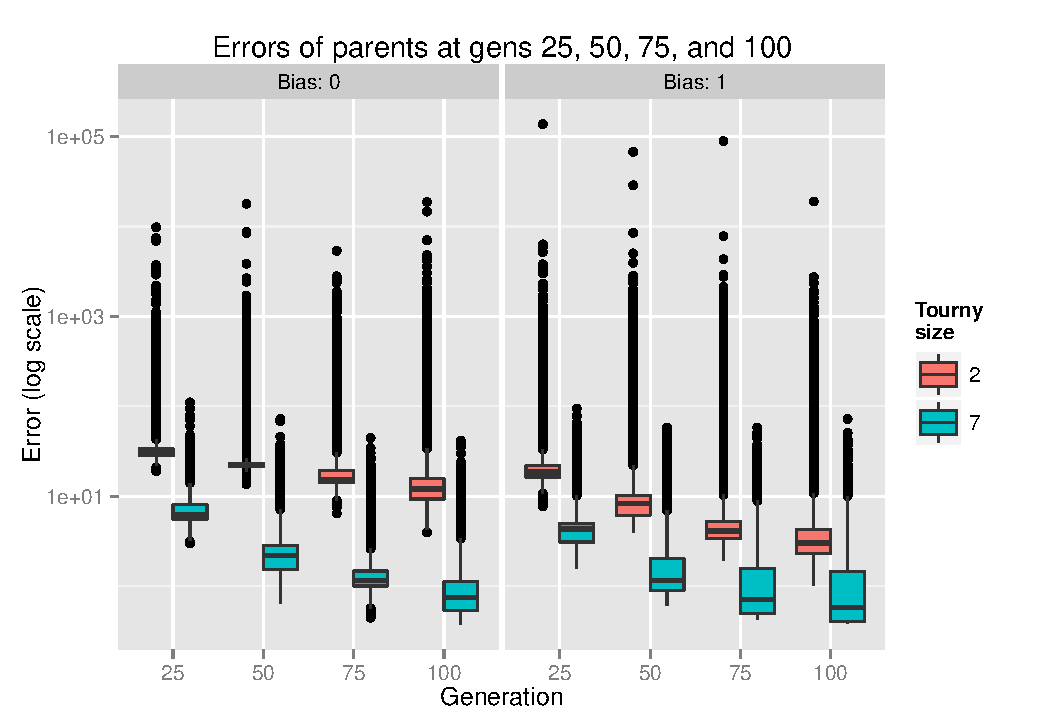
\includegraphics[width=0.45 \textwidth]{Plots/Parent_errors_sine.pdf}
\caption{Plot of the errors of all individuals chosen as parents from some sine runs. \textbf{Explain this.} \textbf{Do we want/need this plot?}}
\label{fig:parentErrorsSine}
\end{figure}

Figure~\ref{fig:parentDiffsSine} shows the distribution of relative difference in parent errors in the sine regression 
problem. For each crossover event, the relative difference in parent errors is
\[
	|e_A - e_B] / (e_A + e_B)
\]
where $e_A$ and $e_B$ are the errors of the two chosen parents $A$ and $B$. This has a minimum value of 0 when 
the two errors are the same, and a maximum value approaching 1 for the case where one of the errors is nearly 0.

\begin{figure}
\centering
\includegraphics[width=0.45 \textwidth]{Plots/Parent_normalized_error_diffs_sine.pdf}
\caption{Plot of the normalized differences in parent errors from some sine runs. \textbf{Explain this}.}
\label{fig:parentDiffsSine}
\end{figure}

We see similar results for the K-Landscapes problem, as illustrated in Figures~\ref{fig:parentFitnessesKLandscapes} and~\ref{fig:parentDiffsKLandscapes}.

\begin{figure}
\centering
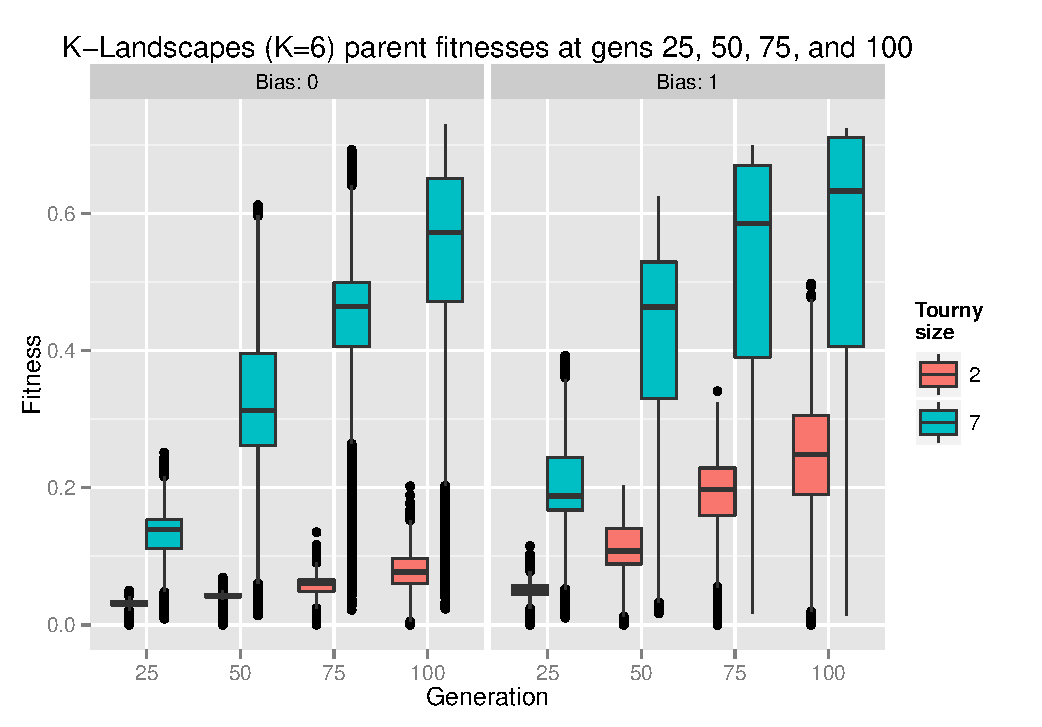
\includegraphics[width=0.45 \textwidth]{Plots/Parent_fitnesses_KLandscapes.pdf}
\caption{Plot of the fitnesses of all individuals chosen as parents from some K-Landscape runs. \textbf{Explain this.} \textbf{Do we want/need this plot?}}
\label{fig:parentFitnessesKLandscapes}
\end{figure}

\begin{figure}
\centering
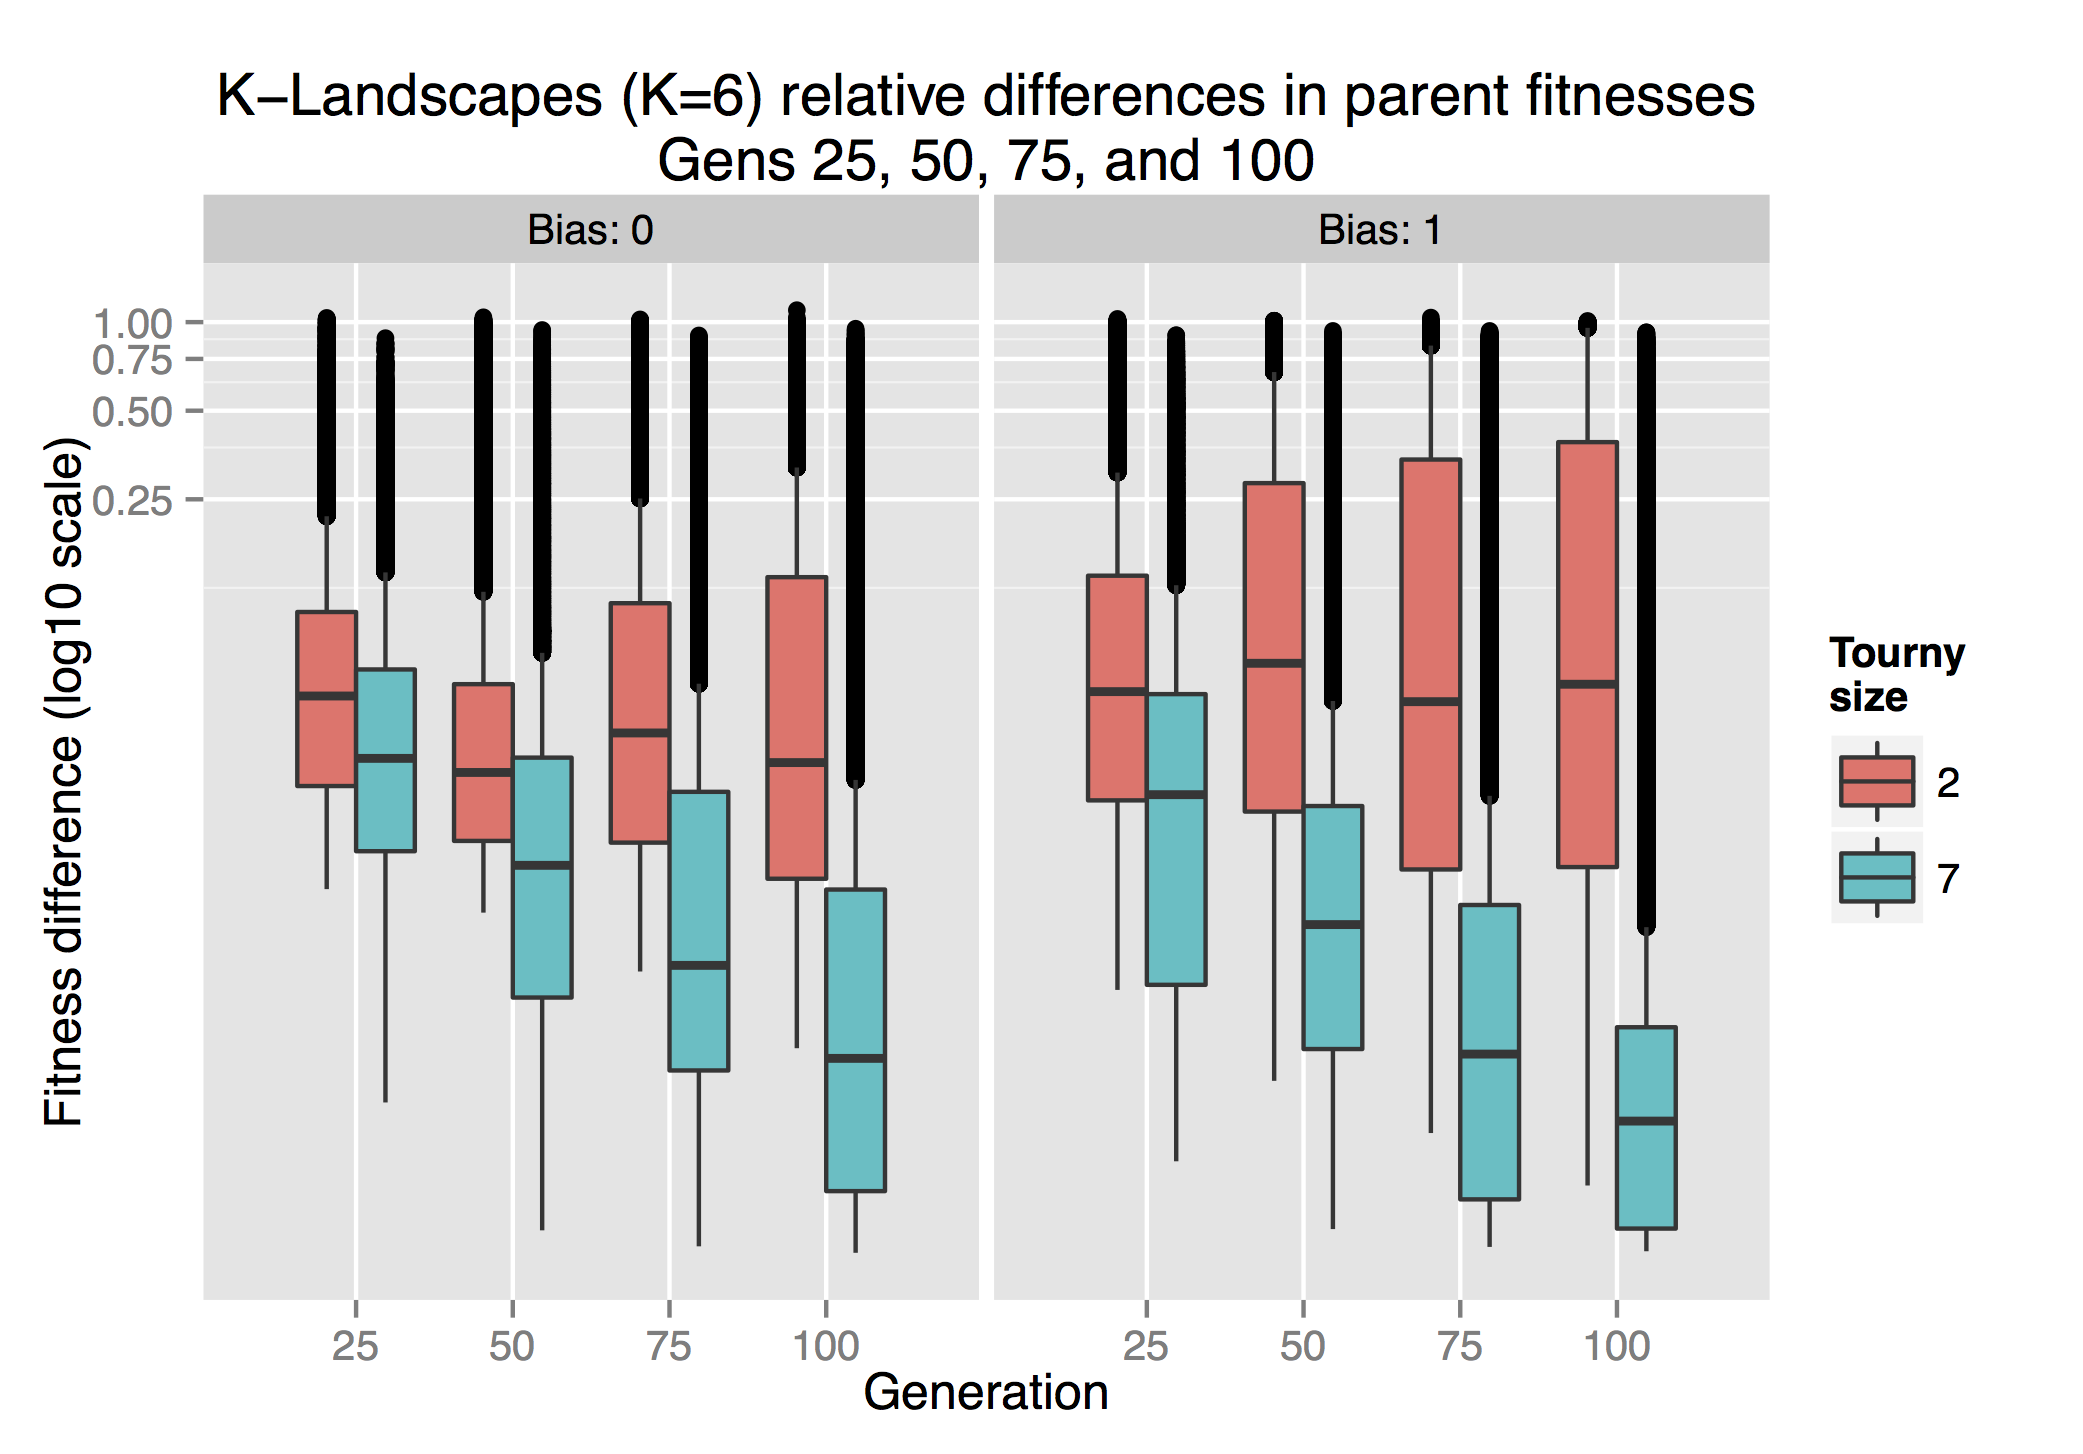
\includegraphics[width=0.45 \textwidth]{Plots/Parent_normalized_fitness_diffs_KLandscapes.pdf}
\caption{Plot of the normalized differences in parent fitnesses from some K-Landscape runs. \textbf{Explain this}.}
\label{fig:parentDiffsKLandscapes}
\end{figure}

\section{Conclusions} \label{sec:Conclusions}

In most of these experiments we found better results with tournament sizes of 7 than with binary tournaments, and in 
general using larger tournaments appears to wash out much of the impact of crossover bias, so there's a fair question 
about whether one should just use larger tournaments and ignore crossover bias. \textbf{How do we respond to this? I 
think the answer is something like ``It doesn't hurt (at least in our experiments), and it sometimes helps, even for 
tournament size 7 and with elitism. For interesting problems, you also don't know in advance what your best parameter 
choices are, so it's at least worth including in your arsenal.''}

\section*{Acknowledgements}

\bibliographystyle{acm}
\bibliography{Research_2015}

\end{document}